\part{Cognition and Information Processing}
\frame{\partpage}

\begin{frame}{Learning Outcomes}
	In this section you will learn how to...
	
	\begin{itemize}
		\item \textbf{Explain} what is meant by `cognition'
		\item \textbf{Show} the importance of information processing models to HCI
		\item \textbf{Explain} the shortcomings of cognitive and information processing models
		\item \textbf{Discuss} the role of cognitive models in games, and HCI more broadly
	\end{itemize}
\end{frame}

\begin{frame}{Further Reading}
	\begin{itemize}
		\item Eysenck, M.W. and Keane, M.T. (2000) \textit{Cognitive Psychology: A Student's Handbook}. 4th Edition. Erlbaum Associatates.
		\item Preece, J., Rogers, Y., Sharp, H., Benyon, D., Holland, S., and Carey, T. (1994) \textit{Human-Computer Interaction}. Addison-Wesley.
	\end{itemize}
\end{frame}

\begin{frame}{What is Cognition?}
	\begin{itemize}
		\item The cognitive approach is currently the dominant framework (or paradigm) for HCI (Perry, 2006).
		\item Players are characterised as `information processors', in which information undergoes a series of ordered processes
		in the player's mind.
		\item This worldview draws a comparison between the human brain and a computer; we can therefore model player activity in the same
		way that we model computer processing.
	\end{itemize}
\end{frame}

\begin{frame}[fragile]{Socrative \texttt{JBYPC3BBY}}
	\begin{itemize}
		\item In pairs.
		\item Quietly discuss what you think is meant by the term `cognition' for 2-minutes.
		\item \textbf{Explain} cognition in your own words.
	\end{itemize}
\end{frame}

\begin{frame}{What is Cognition?}
	\begin{itemize}
		\item Cognition itself refers to the `processes by which we gain knowledge' (Perry, 2006, p. 8).
		
		\vspace{2ex}
		
		\item This includes understanding, remembering, reasoning, attending to, awareness and acquiring skills.
	\end{itemize}
\end{frame}

\begin{frame}{What is Cognition?}
	In a simple model of cognition, such as that proposed by Barber (1988), the process of cognition can be described as composing four sequential
	stages: 
	
	\vspace{2ex}

	\begin{itemize}
		\item Information entering the system as \textbf{input} is first encoded and turned from a physical environment event (i.e., pixels on the screen) 
		into a \textbf{mental representation} held electrochemically in the brain.
		
		\vspace{2ex}
		
		\item This encoded information is then compared to existing repesentations stored in memory.
	\end{itemize}
\end{frame}

\begin{frame}{What is Cognition?}
	In a simple model of cognition, such as that proposed by Barber (1988), the process of cognition can be described as composing four sequential
	stages: 
	
	\vspace{2ex}

	\begin{itemize}
		\item Having compared the representation to the information represented in the memory, the information processor can select an appropriate response.
		
		\vspace{2ex}
		
		\item The final stage involves the execution of the selected response.
	\end{itemize}
\end{frame}

\begin{frame}{What is Cognition?}
	In a simple model of cognition, such as that proposed by Barber (1988), the process of cognition can be described as composing four sequential
	stages: 
	
	\vspace{2ex}

	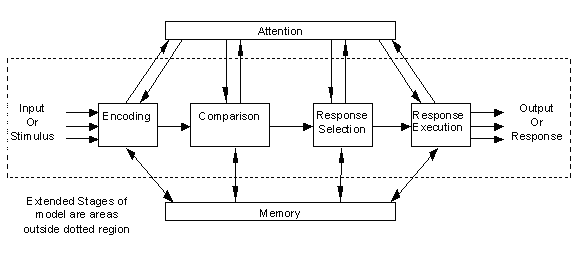
\includegraphics[height=24ex]{barber_cognition.png}
\end{frame}

\begin{frame}[fragile]{Socrative \texttt{JBYPC3BBY}}
	\begin{itemize}
		\item In pairs.
		\item Quietly revisit what is meant by the term `cognition' for 2-minutes.
		\item \textbf{Explain} cognition in your own words.
	\end{itemize}
\end{frame}

\begin{frame}{Cognitve Models in HCI}
	\begin{itemize}
		\item It is important to note that cognitive activity is often conceptualised as being `goal orientated'
		\item This means there is an intended and planned result for the processing.
		\item Or, in other words, `means end analysis' --- determining the difference between the current-state and the goal-state (e.g. interpret current position
		and move towards a power-up, in order to collect it)
	\end{itemize}
\end{frame}

\begin{frame}{Cognitive Models in HCI}
	Newman and Lamming (1995) somewhat controversially called moelling human behaviour in this manner `human virtual machines', drawing from the 
	term `virtual machine', which is a description of an abstract system. 
\end{frame}

\begin{frame}{Cognitive Models in HCI}
	However, as previously illustrated, they have much utility:
	
	\vspace{2ex}

	\begin{itemize}
		\item Understand information requirements needed to identify and progress toward a goal
		\item Optimise representations that are easy for people to encode and compare (e.g. health bar vs absolute number);
		\item Make predictions which can be used to test the efficacy of a design
		\item and so on...
	\end{itemize}
\end{frame}

\begin{frame}{Cognitive Models in HCI}
	Or more generally:
	
	\vspace{2ex}

	\begin{itemize}
		\item Understand what is going on when users use systems
		\item Predict in advance how users will behave
		\item Identify and explain the nature of problems that users encounter
		\item Provide knowledge about what users can and can't be expected to do
		\item Design systems to take advantage of partucular aspects of user skills and abilities
	\end{itemize}
\end{frame}

\begin{frame}{Cognitive Models in HCI}
	There are, however, several drawbacks:
	
	\vspace{2ex}

	\begin{itemize}
		\item An idealised information processing unit is assumed --- people are not so ideal
		\item Individual and ephemeral factors such as motivation and mood play an important role in behaviour;
		\item Considerable variation in characterisitcs and abilities
		\item The system boundary may ignore real-world tools and contexts (e.g. using a DPS calculator instead of performing mental arithmetic manually).
	\end{itemize}
\end{frame}

\begin{frame}[fragile]{Socrative \texttt{JBYPC3BBY}}
	\begin{itemize}
		\item In pairs.
		\item Quietly discuss how cognitive models could inform the design of a game interface.
		\item \textbf{List} the possible uses.
	\end{itemize}
\end{frame}
